% ============================================================
%  Chapter 20 — Optimization Under Uncertainty
%  Algorithms for Optimization, 2nd ed. (2026)
%  Kochenderfer & Wheeler
%  Beamer slides — pdflatex compatible
% ============================================================
\documentclass[aspectratio=169,10pt]{beamer}

\usetheme{Madrid}
\usecolortheme{seahorse}
\setbeamertemplate{footline}[frame number]

% ── packages ────────────────────────────────────────────────
\usepackage{amsmath,amssymb,amsfonts}
\usepackage{bm}
\usepackage{graphicx}
\usepackage{booktabs}
\usepackage{listings}
\usepackage{xcolor}
\usepackage{tikz}
\usepackage{array}
\usepackage{hyperref}

\graphicspath{{figures/}}

% ── listings style ──────────────────────────────────────────
\definecolor{codegray}{gray}{0.93}
\lstset{
  language=Python,
  basicstyle=\ttfamily\scriptsize,
  numbers=left,
  numberstyle=\tiny\color{gray},
  frame=single,
  backgroundcolor=\color{codegray},
  keywordstyle=\color{blue!80!black}\bfseries,
  commentstyle=\color{green!50!black}\itshape,
  stringstyle=\color{orange!80!black},
  showstringspaces=false,
  tabsize=4,
  breaklines=true,
  breakatwhitespace=true,
  numbersep=6pt,
}

% ── convenience macros ──────────────────────────────────────
\newcommand{\x}{\mathbf{x}}
\newcommand{\z}{\mathbf{z}}
\newcommand{\R}{\mathbb{R}}
\newcommand{\E}{\mathbb{E}}
\newcommand{\Var}{\mathrm{Var}}
\newcommand{\T}{\top}
\newcommand{\Norm}{\mathcal{N}}
\newcommand{\Z}{\mathcal{Z}}
\newcommand{\eps}{\epsilon}
\DeclareMathOperator*{\minimize}{minimize}
\DeclareMathOperator*{\maximize}{maximize}

% ── title ───────────────────────────────────────────────────
\title[Ch.\,20: Optimization Under Uncertainty]{%
  Chapter 20\\[4pt]
  \textbf{Optimization Under Uncertainty}}
\subtitle{Algorithms for Optimization, 2nd Edition (2026)}
\author{Kochenderfer \& Wheeler}
\date{Slides prepared for lecture}

% ============================================================
\begin{document}
% ============================================================

\begin{frame}
  \titlepage
\end{frame}

% ── outline ─────────────────────────────────────────────────
\begin{frame}{Chapter Overview}
  \tableofcontents
\end{frame}

\AtBeginSection[]{%
  \begin{frame}{Outline}
    \tableofcontents[currentsection]
  \end{frame}
}

% ============================================================
\section{Types of Uncertainty}
% ============================================================

\begin{frame}{Why Uncertainty Matters}
  \begin{columns}
    \column{0.55\textwidth}
      \begin{block}{Core Problem}
        Previous chapters assumed the objective function
        $f(\x)$ is \emph{deterministic}.\\[4pt]
        In practice, uncertainty arises from:
        \begin{itemize}
          \item \textbf{Model error} — imperfect mathematical model
          \item \textbf{Manufacturing tolerances} — built design deviates from nominal
          \item \textbf{Environmental variation} — operating conditions change
          \item \textbf{Measurement noise} — noisy sensor readings
          \item \textbf{Distributional shift} — unknown inputs at test time
        \end{itemize}
      \end{block}
    \column{0.42\textwidth}
      \centering
      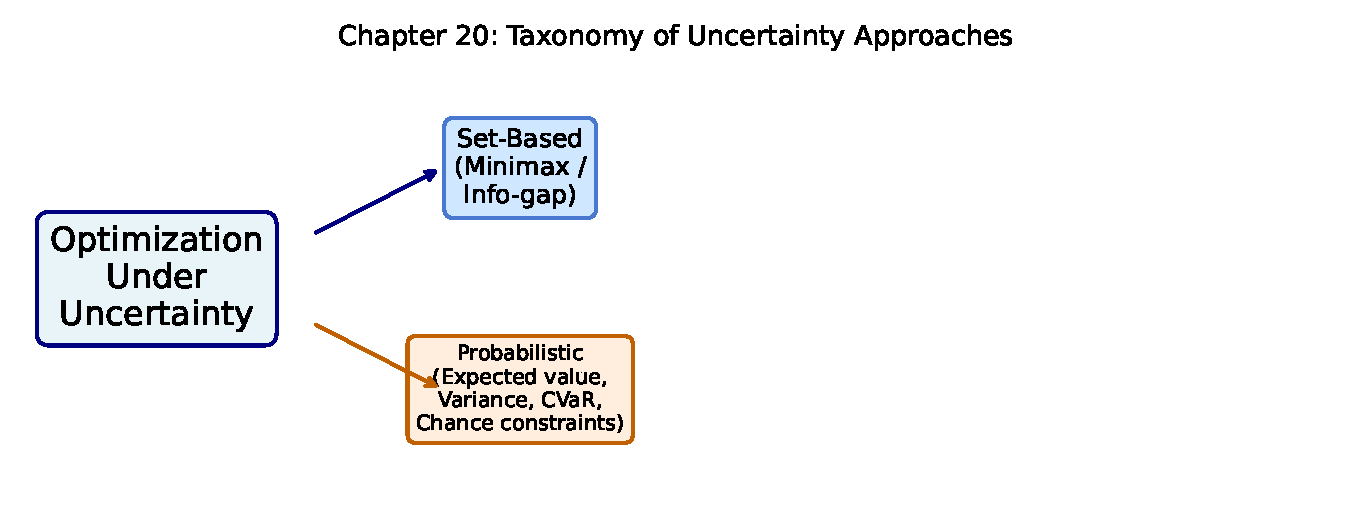
\includegraphics[width=\textwidth]{uncertainty_types}\\[2pt]
      {\scriptsize Two main paradigms: set-based and probabilistic}
  \end{columns}
\end{frame}

\begin{frame}{Uncertain Objective Function}
  \begin{block}{General Formulation}
    The objective depends on a \textbf{design vector} $\x \in \R^n$
    and an \textbf{uncertainty vector} $\z \in \R^m$:
    \[
      \text{minimize}_{\x} \quad f(\x, \z)
    \]
    Uncertainty $\z$ cannot be controlled but may have known properties.
  \end{block}

  \begin{columns}
    \column{0.55\textwidth}
      \textbf{Running example (p.\,428):}\\
      We evaluate $f(\x, \z) = f(\x + \z) = f(\tilde{x})$\\
      where $\tilde{x} = x + z$.\\[4pt]
      \begin{itemize}
        \item $z$ may come from a \emph{Gaussian distribution} $\mathcal{N}(0,\nu)$
        \item Expected value: $\E_{\z}[f(\x+\z)] \ne f(\x)$ in general
        \item Variance of $z$ changes optimal design location
      \end{itemize}
    \column{0.42\textwidth}
      \centering
      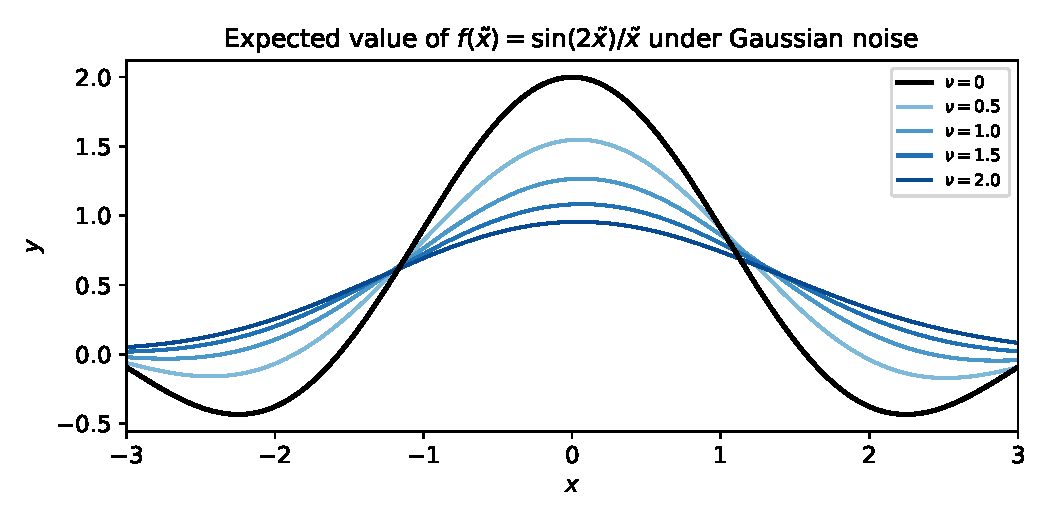
\includegraphics[width=\textwidth]{noisy_objective}\\[-2pt]
      {\scriptsize Objective $f(\tilde{x})=\sin(2\tilde{x})/\tilde{x}$ under varying noise}
  \end{columns}
\end{frame}

\begin{frame}{Two Paradigms for Handling Uncertainty}
  \begin{columns}
    \column{0.48\textwidth}
      \begin{alertblock}{Set-Based Uncertainty}
        $z$ belongs to a \emph{known set} $\Z$:\\[4pt]
        $\z \in \Z$\\[4pt]
        \textbf{No probability distribution assumed.}\\[4pt]
        Approaches:
        \begin{itemize}
          \item \textbf{Minimax} — optimize worst case
          \item \textbf{Info-gap} — maximize robustness radius
        \end{itemize}
        Natural when: physical bounds are known but
        statistics are not.
      \end{alertblock}
    \column{0.48\textwidth}
      \begin{block}{Probabilistic Uncertainty}
        $\z$ is drawn from a distribution $P$:\\[4pt]
        $\z \sim P$\\[4pt]
        \textbf{Probability distribution is modeled.}\\[4pt]
        Approaches:
        \begin{itemize}
          \item \textbf{Expected value} minimization
          \item \textbf{Variance} / mean-variance trade-off
          \item \textbf{CVaR} — conditional value at risk
          \item \textbf{Chance constraints} — probabilistic feasibility
        \end{itemize}
      \end{block}
  \end{columns}
\end{frame}

% ============================================================
\section{Set-Based Uncertainty (Minimax)}
% ============================================================

\begin{frame}{Set-Based Uncertainty — Setup}
  \begin{block}{Assumption}
    Set-based uncertainty assumes $\z$ belongs to a \emph{set} $\Z \subset \R^m$.
    No probability distribution is assumed.\\[4pt]
    One way to define $\Z$: use \textbf{interval constraints} on each component:
    \[
      z_i \in [a_i,\, b_i] \quad \text{for all } i
    \]
  \end{block}
  \vspace{4pt}
  \begin{block}{Alternative: Inequality Constraints}
    $\Z$ can also be defined via a set of inequalities:
    \[
      \Z = \{\z : g_j(\z) \leq 0,\; j = 1,\dots,m\}
    \]
    e.g., ellipsoidal uncertainty sets.
  \end{block}
  \vspace{4pt}
  Goal: find a design that performs well \textbf{for any} $\z \in \Z$.
\end{frame}

\begin{frame}{20.2.1 \; Minimax}
  \begin{block}{Minimax Formulation}
    The \textbf{minimax} approach minimizes the worst-case objective:
    \[
      \boxed{\minimize_{\x} \; f_{\mathrm{mod}}(\x)
        \quad \text{where} \quad
        f_{\mathrm{mod}}(\x) = \maximize_{\z \in \Z}\; f(\x, \z)}
    \]
    \smallskip
    \begin{tabular}{ll}
      $f_{\mathrm{mod}}(\x)$ & modified objective (worst-case value)\\
      $\Z$                   & uncertainty set\\
    \end{tabular}
  \end{block}
  \begin{itemize}
    \item Equivalent to a \textbf{nested} min-over-max optimization
    \item If $f$ and $\Z$ are convex, the outer problem is convex
    \item With feasibility constraints: restrict to designs feasible \emph{for all} $\z \in \Z$
  \end{itemize}
\end{frame}

\begin{frame}{Minimax Example (Example 20.1)}
  \begin{columns}
    \column{0.52\textwidth}
      \begin{block}{Setup}
        \[
          f(x,z) = f(\tilde{x}),\quad \tilde{x} = x+z
        \]
        \[
          f(\tilde{x}) = \begin{cases} -\tilde{x} & \tilde{x} \le 0 \\ \tilde{x}^2 & \text{otherwise}\end{cases}
        \]
        Uncertainty set: $z \in [-\eps, \eps]$\\[4pt]
        Minimax objective:
        \[
          f_{\mathrm{mod}}(x) = \max_{z \in [-\eps,\eps]} f(x+z)
        \]
      \end{block}
      \begin{itemize}
        \item $\eps=0$: minimizer at $x^* = 0$
        \item As $\eps$ increases, minimizer shifts
        \item Robust minimizer $\ne$ noise-free minimizer
      \end{itemize}
    \column{0.45\textwidth}
      \centering
      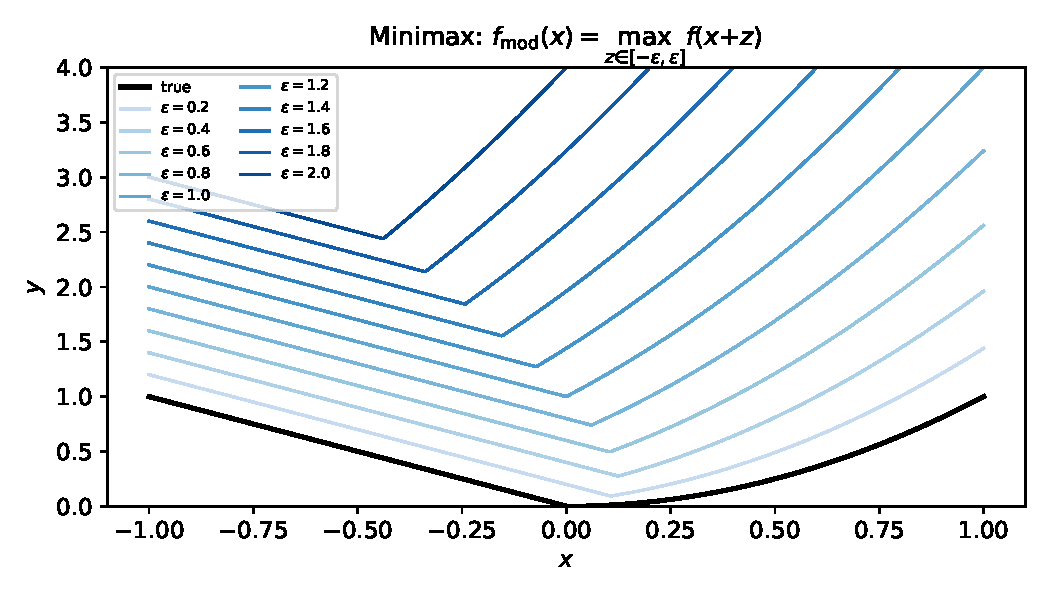
\includegraphics[width=\textwidth]{minimax_fmod}\\[-2pt]
      {\scriptsize $f_{\mathrm{mod}}(x)$ for $\eps = 0,0.2,\ldots,2.0$}
  \end{columns}
\end{frame}

\begin{frame}{Minimax with Feasibility Constraints}
  \begin{block}{Robust Feasibility}
    In problems with constraints $(\x, \z) \in \mathcal{F}$,
    a minimax approach considers only designs
    \textbf{feasible for all} $\z \in \Z$:
    \[
      \minimize_{\x} \; f_{\mathrm{mod}}(\x) \quad
      \text{s.t.} \quad (\x, \z) \in \mathcal{F} \;\;\forall\, \z \in \Z
    \]
    Equivalently, the robust feasible set is the \textbf{intersection}:
    \[
      \mathcal{F}_{\mathrm{robust}} = \bigcap_{\z \in \Z} \mathcal{F}_z
    \]
  \end{block}
  \begin{columns}
    \column{0.52\textwidth}
      \textbf{Example 20.2 — Rotated Ellipse:}\\
      $(\x,z) \in \mathcal{F}$ iff $z \in [0,\pi/2]$ and
      \[
        (x_1 \cos z + x_2 \sin z)^2
        + \frac{(x_1 \sin z - x_2 \cos z)^2}{16} \le 1
      \]
      \textbf{Blue}: union (feasible for some $z$)\\
      \textbf{Red}: intersection (robust feasible set)
    \column{0.45\textwidth}
      \centering
      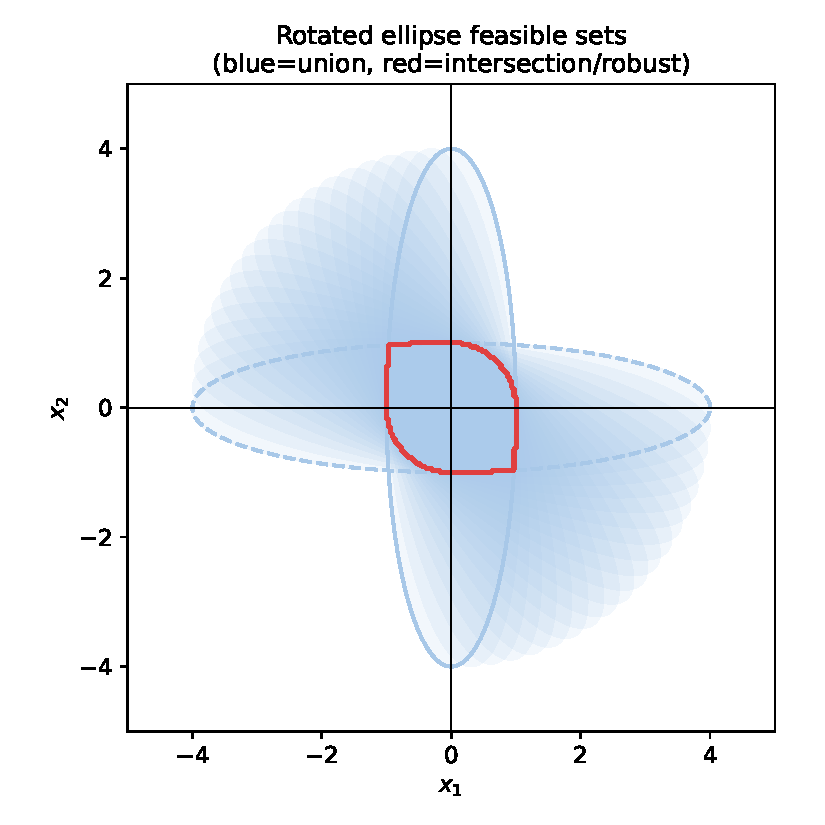
\includegraphics[width=\textwidth]{rotated_ellipse}
  \end{columns}
\end{frame}

\begin{frame}{20.2.2 \; Information-Gap Decision Theory}
  \begin{block}{Alternative to Minimax}
    Instead of fixing $\Z$ and minimizing $f_{\mathrm{mod}}$,
    \textbf{info-gap decision theory} asks:
    \emph{how large can $\Z$ be while still achieving an acceptable objective value?}\\[6pt]
    Given a \textbf{performance requirement} $f_c$, find:
    \[
      \hat{\eps}(\x) = \maximize_{\eps \geq 0}\left\{
        \eps : \max_{\z \in \Z(\eps)} f(\x,\z) \leq f_c
      \right\}
    \]
    \begin{tabular}{ll}
      $\hat{\eps}(\x)$ & robustness radius of design $\x$ \\
      $\Z(\eps)$       & uncertainty set of size $\eps$ \\
      $f_c$            & critical (acceptable) objective value \\
    \end{tabular}
  \end{block}
  \vspace{4pt}
  \textbf{Key idea:} Maximize the \emph{robustness horizon} — the largest perturbation
  tolerable while maintaining acceptable performance.
\end{frame}

\begin{frame}{Info-Gap: Example 20.3}
  \begin{columns}
    \column{0.52\textwidth}
      \begin{block}{Problem}
        $f(x,z) = \tilde{x}^2 + 6e^{-\tilde{x}^2}$,\; $\tilde{x}=x+z$\\
        $\tilde{x} \in [-2,2]$,\; $\Z(\eps) = [-\eps,\eps]$
      \end{block}
      \vspace{4pt}
      \textbf{Top panel}: Unconstrained info-gap.\\
      Pure info-gap centers on a \emph{suboptimal} region —
      risk aversion is excessive.\\[4pt]
      \textbf{Bottom panel}: With constraint $f(x,z) \le 5$.\\
      Adding a performance bound moves $x^*$ to a
      region with \emph{better} noise-free performance.\\[4pt]
      Blue lines = worst-case objective value for each $\eps$.
    \column{0.45\textwidth}
      \centering
      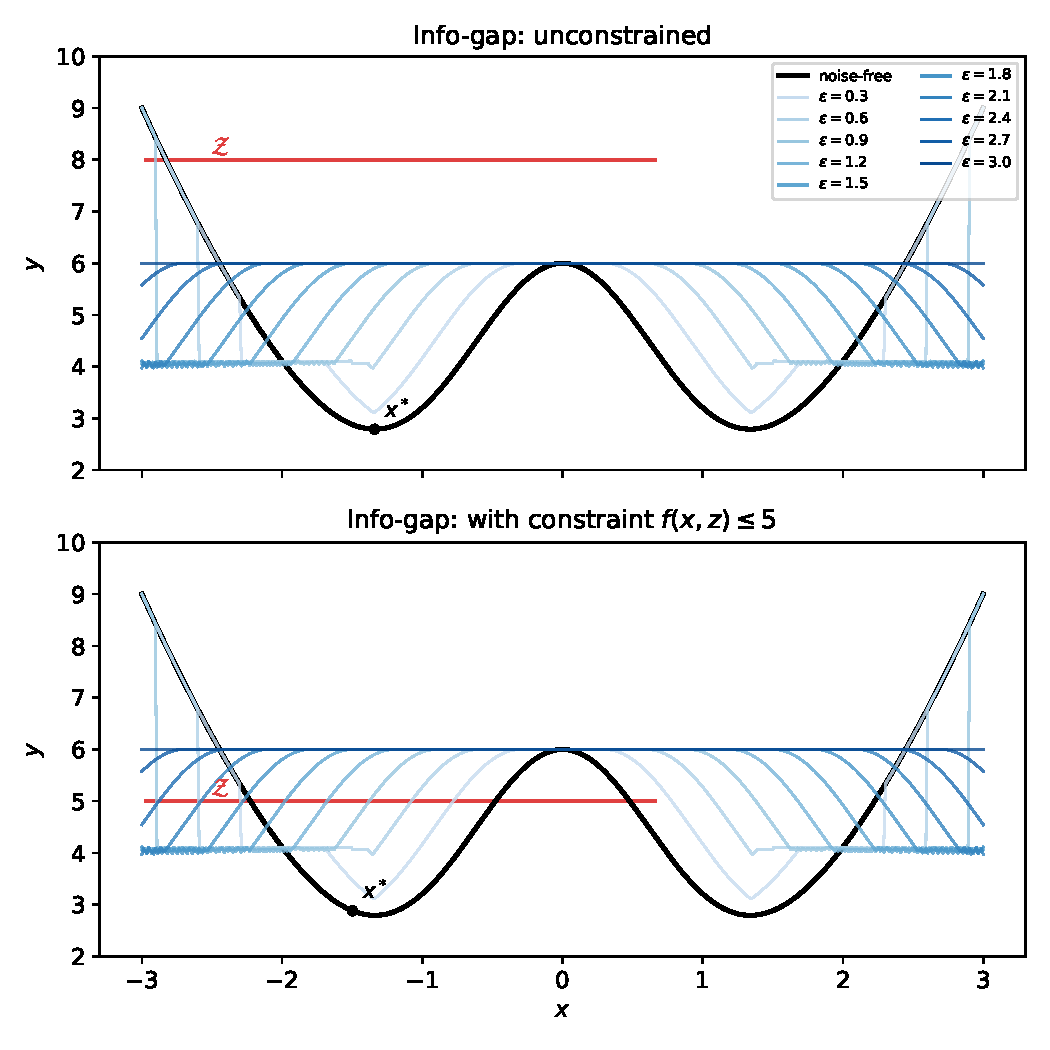
\includegraphics[width=0.95\textwidth]{info_gap}
  \end{columns}
\end{frame}

\begin{frame}[fragile]{Python: Minimax Optimization}
\begin{lstlisting}
import numpy as np
from scipy.optimize import minimize, differential_evolution

def f_tilde(xtilde):
    """Piecewise objective f(x+z)."""
    return np.where(xtilde <= 0, -xtilde, xtilde**2)

def f_mod(x, eps, n_z=200):
    """Worst-case objective over z in [-eps, eps]."""
    z_vals = np.linspace(-eps, eps, n_z)
    return np.max(f_tilde(x + z_vals))

# Minimax: minimize worst-case over x in [-1, 1]
eps = 0.5
result = minimize(
    lambda x: f_mod(x[0], eps),
    x0=[0.0],
    method='L-BFGS-B',
    bounds=[(-1, 1)]
)
x_robust = result.x[0]
print(f"Robust minimizer (eps={eps}): x* = {x_robust:.4f}")
# eps=0.5 -> x* shifts right from 0 toward positive values
\end{lstlisting}
\vspace{2pt}
{\small Minimax requires evaluating $f$ over the full uncertainty set $\Z$ at each $\x$ — computationally more expensive than noise-free optimization.}
\end{frame}

% ============================================================
\section{Probabilistic Uncertainty}
% ============================================================

\begin{frame}{20.3 \; Probabilistic Uncertainty — Overview}
  \begin{block}{Setup}
    Assume $\z$ is drawn from a \textbf{probability distribution} $P$:
    \[
      \z \sim P(\z)
    \]
    The objective $f(\x, \z)$ is now a \emph{random variable} $y = f(\x, \z)$.\\[6pt]
    We optimize over the distribution of $y$ using various risk measures:
  \end{block}
  \vspace{6pt}
  \begin{columns}
    \column{0.5\textwidth}
      \begin{enumerate}
        \item \textbf{Expected value:}\quad $\E_\z[f(\x,\z)]$
        \item \textbf{Variance:}\quad $\Var_\z[f(\x,\z)]$
        \item \textbf{Mean-variance trade-off:} combined
        \item \textbf{Value at Risk (VaR):} quantile
        \item \textbf{Conditional Value at Risk (CVaR):} tail mean
        \item \textbf{Chance constraints:} $\Pr[g(\x,\z)\le 0] \ge 1-\delta$
      \end{enumerate}
    \column{0.47\textwidth}
      \centering
      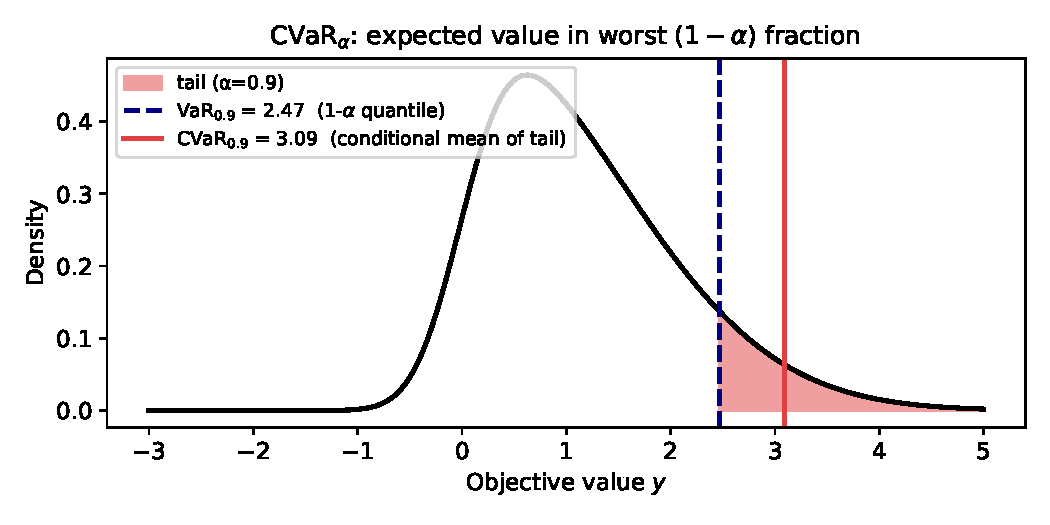
\includegraphics[width=\textwidth]{cvar_quantile}\\
      {\scriptsize VaR vs CVaR on a distribution of objective values}
  \end{columns}
\end{frame}

\begin{frame}{20.3.1 \; Expected Value}
  \begin{block}{Expected Value Objective}
    \[
      \boxed{\minimize_{\x}\; \E_{\z\sim P}\bigl[f(\x,\z)\bigr]
        = \minimize_{\x}\; \int f(\x,\z)\, P(\z)\, d\z}
    \]
    \begin{tabular}{ll}
      $P(\z)$         & probability density / distribution of uncertainty \\
      $f(\x,\z)$      & objective under uncertainty realization $\z$ \\
    \end{tabular}
  \end{block}
  \vspace{4pt}
  \textbf{Key properties:}
  \begin{itemize}
    \item If $f(\x,\z) = f(\x) + \z$ (additive noise), then
          $\E[f(\x,\z)] = f(\x) + \E[\z]$ — noise shifts value, not optimum
    \item If $f(\x,\z) = f(\x+\z) = f(\tilde{x})$, the expected value
          \emph{smooths} the landscape (regularization effect)
    \item Zero-mean Gaussian output noise:
          $\E_{\z\sim\Norm(0,\Sigma)}[f(\x)+\z] = f(\x)$ — \emph{no effect}
    \item Zero-mean Gaussian input noise \emph{does} shift optima
  \end{itemize}
\end{frame}

\begin{frame}{Expected Value: Gaussian Input Noise (Example 20.4)}
  \begin{columns}
    \column{0.50\textwidth}
      \begin{block}{Setup}
        Minimize $\E[f(\tilde{x})]$ where $f(\tilde{x}) = \sin(2\tilde{x})/\tilde{x}$\\
        with $\tilde{x} = x + z$, $z \sim \Norm(0,\nu)$\\[4pt]
        Zero-mean output noise: $\E[f(\x)+\z] = f(\x)$\\
        (no effect on objective)\\[4pt]
        Zero-mean \emph{input} noise: \emph{affected by} $\nu$
        \[
          \E_{\z\sim\Norm(\mathbf{0},\Sigma)}[f(\x)+\z] = f(\x)
        \]
        \[
          \E_{\z\sim\Norm(\mathbf{0},\Sigma)}[f(\x+\z)] \ne f(\x)
        \]
      \end{block}
      Increasing $\nu$ smooths the landscape:\\
      local optima are averaged out.
    \column{0.47\textwidth}
      \centering
      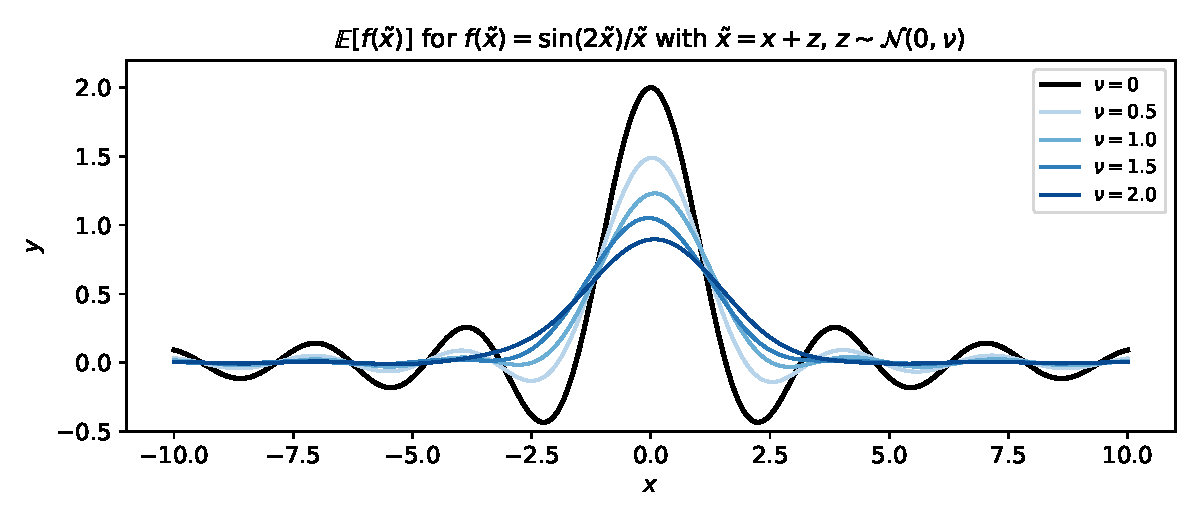
\includegraphics[width=\textwidth]{expected_value_gaussian}\\
      {\scriptsize Higher $\nu \Rightarrow$ smoother, shifted optima}
  \end{columns}
\end{frame}

\begin{frame}{20.3.2 \; Variance}
  \begin{block}{Variance as a Risk Measure}
    Variance quantifies \textbf{spread} of the objective around its mean:
    \[
      \Var_{\z}\bigl[f(\x,\z)\bigr]
      = \E\bigl[\bigl(f(\x,\z) - \E[f(\x,\z)]\bigr)^2\bigr]
    \]
    Minimizing variance alone tends to over-penalize large deviations;
    often \textbf{combined with the mean}:
    \[
      \minimize_{\x}\;\; \alpha\,\E[f(\x,\z)]
        + (1-\alpha)\sqrt{\Var[f(\x,\z)]}
      \quad \alpha \in [0,1]
    \]
    \begin{tabular}{ll}
      $\alpha=1$   & pure expected-value optimization \\
      $\alpha=0$   & pure variance minimization \\
      $0<\alpha<1$ & trade-off between mean and spread \\
    \end{tabular}
  \end{block}
\end{frame}

\begin{frame}{Variance Example (Example 20.5)}
  \begin{columns}
    \column{0.48\textwidth}
      \begin{block}{Problem}
        $f(x,z) = x^2 + z$, \;
        $z \sim \mathrm{Gamma}\!\left(\tfrac{2}{1+|x|}, 2\right)$\\[4pt]
        Mean: $\E[z\mid x] = \dfrac{4}{1+|x|}$\\[4pt]
        Variance: $\Var[z\mid x] = \dfrac{8}{1+|x|}$\\[4pt]
        Expected objective: $\E[f] = x^2 + \dfrac{4}{1+|x|}$\\[4pt]
        Minima (EV only) at $x \approx \pm 0.695$\\[4pt]
        Adding variance penalty shifts minima \emph{away} from $\pm0.695$.
      \end{block}
    \column{0.48\textwidth}
      \centering
      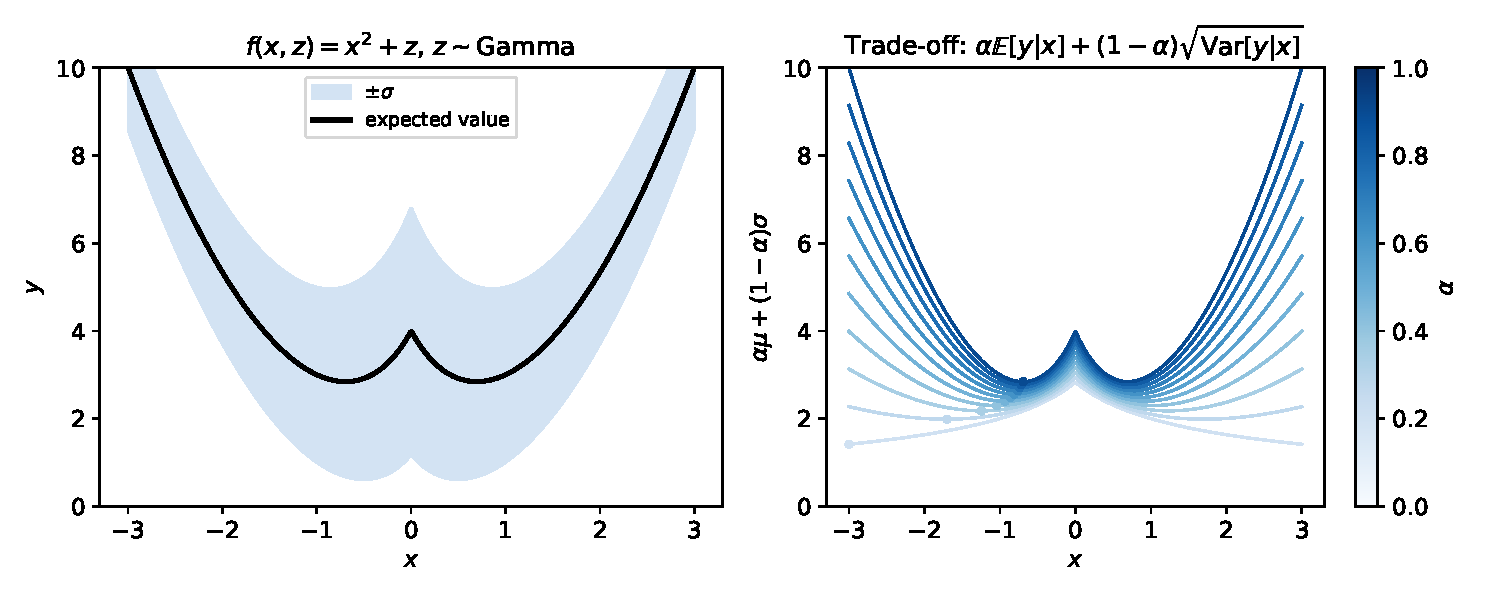
\includegraphics[width=\textwidth]{mean_variance_tradeoff}\\
      {\scriptsize Left: $\pm\sigma$ band; Right: $\alpha$-trade-off}
  \end{columns}
\end{frame}

\begin{frame}{Markowitz Portfolio Optimization (Example 20.6)}
  \begin{columns}
    \column{0.52\textwidth}
      \begin{block}{Mean-Variance in Finance}
        Portfolio $\x$ invests $x_i$ in stock $i$.\\
        Returns $\z \sim \Norm(\bm{\mu}, \bm{\Sigma})$,\;
        portfolio return $y = \x^\T \z$.\\[4pt]
        \textbf{Markowitz problem:}
        \[
          \begin{aligned}
            &\minimize_{\x} \;-w\x^\T\bm{\mu} + (1-w)\x^\T\bm{\Sigma}\x\\
            &\text{s.t.} \quad \x^\T\mathbf{1} = b,\; \x \ge \mathbf{0}
          \end{aligned}
        \]
        \begin{tabular}{ll}
          $\bm{\mu}=[0.26, 0.08, 0.74]^\T$ & expected returns\\
          $w \in [0,1]$ & weight on return vs.\ risk\\
        \end{tabular}\\[4pt]
        This is a \textbf{quadratic program} (Chapter 13).
      \end{block}
    \column{0.45\textwidth}
      \centering
      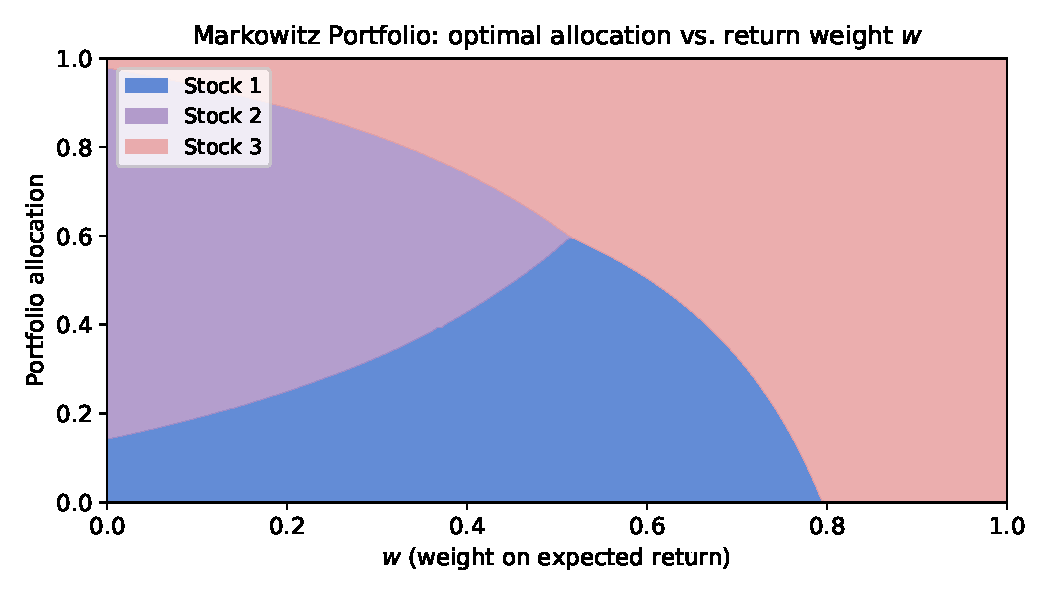
\includegraphics[width=\textwidth]{markowitz_portfolio}\\
      {\scriptsize As $w \to 1$: high-return stock 3 dominates.\\
       As $w \to 0$: low-variance stock 2 dominates.}
  \end{columns}
\end{frame}

\begin{frame}[fragile]{Python: Mean-Variance Portfolio Optimization}
\begin{lstlisting}
import numpy as np
from scipy.optimize import minimize

mu    = np.array([0.26, 0.08, 0.74])
Sigma = np.array([[0.21, 0.03, 0.01],
                  [0.03, 0.06, 0.04],
                  [0.01, 0.04, 0.94]])
b = 1.0  # budget

def markowitz(w):
    """Optimal Markowitz portfolio for return weight w."""
    def obj(x): return -w * x @ mu + (1-w) * x @ Sigma @ x
    def jac(x): return -w * mu + 2*(1-w) * Sigma @ x
    res = minimize(obj, np.ones(3)/3, jac=jac,
                   method='SLSQP',
                   constraints=[{'type':'eq',
                                 'fun': lambda x: x.sum() - b}],
                   bounds=[(0,None)]*3)
    return res.x

# w=1.0: maximize expected return
x_ret  = markowitz(1.0)
# w=0.0: minimize variance
x_safe = markowitz(0.0)
print(f"Max-return portfolio: {x_ret.round(3)}")
print(f"Min-variance portfolio: {x_safe.round(3)}")
\end{lstlisting}
\vspace{2pt}
{\small Using \texttt{scipy.optimize.minimize} with SLSQP for quadratic programming.}
\end{frame}

\begin{frame}{20.3.3 \; Value at Risk (VaR)}
  \begin{block}{Definition}
    The \textbf{Value at Risk} at level $\alpha$ is the $\alpha$-quantile of the
    objective value distribution $y = f(\x,\z)$:
    \[
      \mathrm{VaR}_\alpha(\x) = \inf\bigl\{y : \Pr[f(\x,\z) \le y] \ge \alpha \bigr\}
    \]
    \begin{tabular}{ll}
      $\alpha \in (0,1)$       & confidence level (e.g.\ 0.95)\\
      $\mathrm{VaR}_\alpha$    & objective value exceeded with probability $1-\alpha$\\
    \end{tabular}
  \end{block}
  \vspace{4pt}
  \textbf{Numerical example:} $\alpha = 0.95$, samples of $y = f(\x,\z)$:\\
  \begin{itemize}
    \item $\mathrm{VaR}_{0.95}$ is the 95th percentile of $y$
    \item Only 5\% of outcomes exceed $\mathrm{VaR}_{0.95}$
  \end{itemize}
  \vspace{4pt}
  \textbf{Limitation:} VaR is not coherent — it ignores severity of
  losses \emph{beyond} the quantile threshold.
\end{frame}

\begin{frame}{20.3.4 \; Conditional Value at Risk (CVaR)}
  \begin{columns}
    \column{0.55\textwidth}
      \begin{block}{Definition}
        \textbf{CVaR}$_\alpha$ (also called \emph{expected shortfall} or
        \emph{superquantile}) is the \textbf{expected value of $y$ in the
        worst $(1-\alpha)$ fraction}:
        \[
          \mathrm{CVaR}_\alpha(\x) =
          \frac{1}{1-\alpha}\int_\alpha^1 \mathrm{VaR}_u(\x)\, du
        \]
        Equivalently:
        \[
          \mathrm{CVaR}_\alpha(\x) =
          \E\bigl[f(\x,\z) \mid f(\x,\z) \ge \mathrm{VaR}_\alpha(\x)\bigr]
        \]
      \end{block}
      \textbf{Advantages over VaR:}
      \begin{itemize}
        \item Convex and sub-additive (coherent risk measure)
        \item Less sensitive to estimation errors
        \item Captures severity of extreme outcomes
      \end{itemize}
    \column{0.42\textwidth}
      \centering
      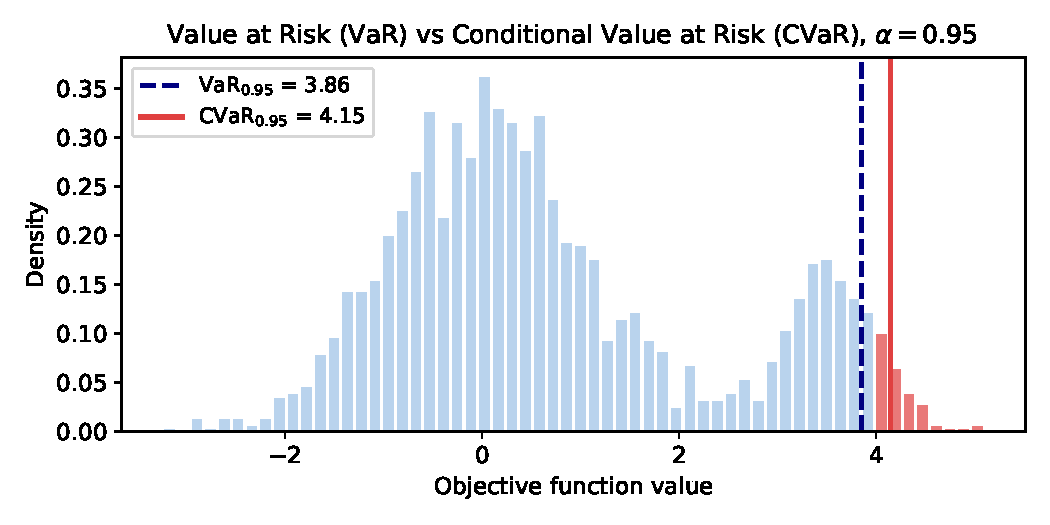
\includegraphics[width=\textwidth]{cvar_var}\\[4pt]
      {\scriptsize Red region = worst $(1-\alpha)$ fraction.\\
       CVaR = mean of red region.}
  \end{columns}
\end{frame}

\begin{frame}{CVaR: Tractable Reformulation}
  \begin{block}{Rockafellar-Uryasev Formula (2000)}
    CVaR admits a tractable optimization formulation:
    \[
      \mathrm{CVaR}_\alpha(\x) = \min_{\tau \in \R}\left\{
        \tau + \frac{1}{1-\alpha}\,\E_\z\bigl[\max(f(\x,\z) - \tau,\, 0)\bigr]
      \right\}
    \]
    \begin{tabular}{ll}
      $\tau$  & auxiliary variable (optimal $\tau^* = \mathrm{VaR}_\alpha$) \\
    \end{tabular}
  \end{block}
  \vspace{4pt}
  \textbf{Key properties:}
  \begin{itemize}
    \item Always $\mathrm{CVaR}_\alpha \ge \mathrm{VaR}_\alpha \ge \E[f]$
    \item CVaR is a \textbf{coherent risk measure}
    \item Monte Carlo estimation: sort samples, take mean of top $(1-\alpha)$
  \end{itemize}
  \vspace{4pt}
  \begin{block}{Numerical Example}
    If $f$ values (sorted) are $[1.0, 1.5, 2.0, 2.5, 3.0, 4.0, 6.0, 8.0, 9.0, 10.0]$
    with $\alpha = 0.90$:\\
    $\mathrm{VaR}_{0.90} = 9.0$,\quad
    $\mathrm{CVaR}_{0.90} = \frac{9.0 + 10.0}{2} = 9.5$
  \end{block}
\end{frame}

\begin{frame}[fragile]{Python: CVaR Estimation and Optimization}
\begin{lstlisting}
import numpy as np
from scipy.optimize import minimize

def cvar_mc(x, f_func, dist_sample, alpha=0.95, n=1000):
    """Monte Carlo CVaR estimate."""
    z_samples = dist_sample(n)                  # shape (n,)
    y = np.array([f_func(x, z) for z in z_samples])
    y_sorted = np.sort(y)
    k = int(np.ceil(alpha * n))                 # index of VaR
    var_alpha  = y_sorted[k]
    cvar_alpha = y_sorted[k:].mean()            # CVaR = mean of tail
    return cvar_alpha, var_alpha

# Example: f(x,z) = (x - z)^2, z ~ N(0,1)
f_func = lambda x, z: (x - z)**2
dist_sample = lambda n: np.random.randn(n)

# Minimize CVaR_0.95 over x in [-3, 3]
def neg_cvar(xvec):
    return cvar_mc(xvec[0], f_func, dist_sample, alpha=0.95)[0]

res = minimize(neg_cvar, [0.0], method='Nelder-Mead',
               options={'xatol':1e-4,'fatol':1e-4})
print(f"CVaR-optimal x = {res.x[0]:.4f}")
# Expect x* near 0 (minimizing expected squared deviation from z~N(0,1))
\end{lstlisting}
\end{frame}

\begin{frame}{20.3.5 \; Statistical Feasibility (Chance Constraints)}
  \begin{block}{Chance Constraint Formulation}
    Instead of requiring $g(\x,\z) \le 0$ for \emph{all} $\z$,
    require feasibility with \textbf{high probability}:
    \[
      \boxed{\Pr_{\z\sim P}\bigl[g(\x,\z) \le 0\bigr] \ge 1 - \delta}
    \]
    \begin{tabular}{ll}
      $\delta \in (0,1)$  & acceptable violation probability \\
      $1-\delta$          & required confidence level \\
    \end{tabular}
  \end{block}
  \vspace{4pt}
  \begin{columns}
    \column{0.50\textwidth}
      \textbf{Approaches:}
      \begin{itemize}
        \item \textbf{Analytical}: closed-form if $\z$ Gaussian and $g$ linear
        \item \textbf{Sample average approximation}: replace $\Pr[\cdot]$ with
              fraction of satisfied samples
        \item \textbf{Factor of safety}: scale constraints $g(\x) \le g_{\max}/\gamma$
              with $\gamma > 1$
      \end{itemize}
    \column{0.46\textwidth}
      \centering
      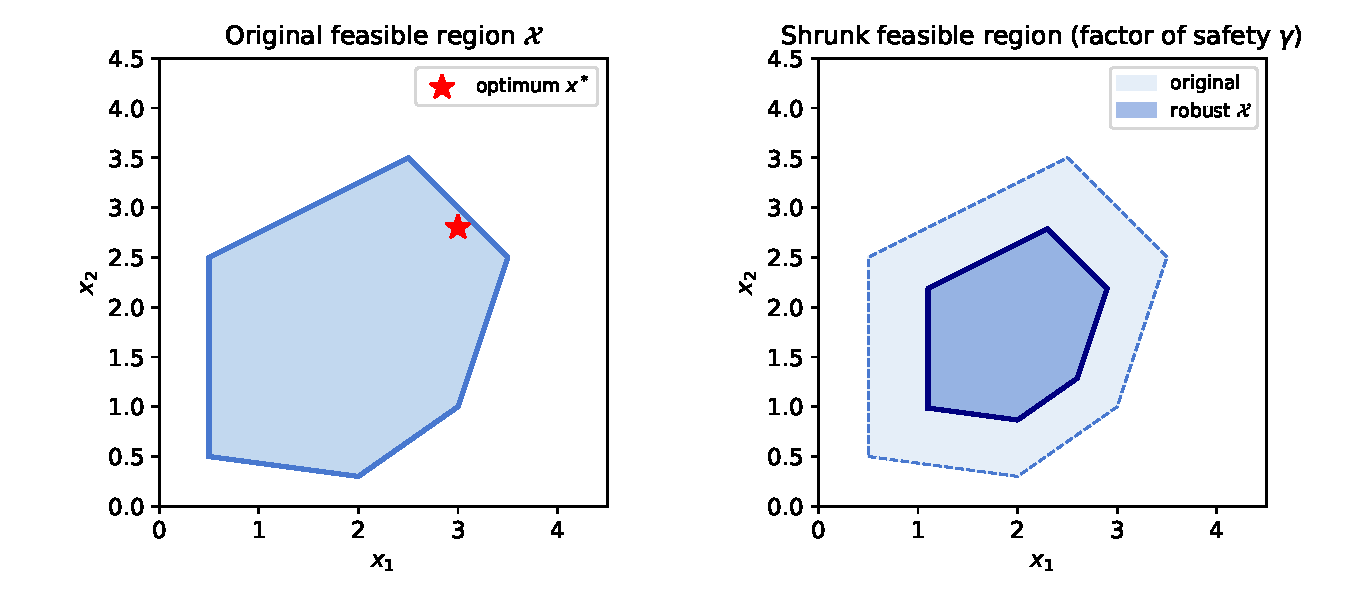
\includegraphics[width=\textwidth]{chance_constraint}\\
      {\scriptsize Shrinking feasible region via factor of safety $\gamma$}
  \end{columns}
\end{frame}

\begin{frame}{Statistical Feasibility: Factor of Safety}
  \begin{block}{Factor of Safety}
    Rewrite constraint $g(\x) \le g_{\max}$ as:
    \[
      \gamma\, g(\x) \le g_{\max}, \quad \gamma > 1
    \]
    where $\gamma$ is the \textbf{factor of safety}.\\[4pt]
    This ensures the design stays below $g_{\max}/\gamma < g_{\max}$,
    providing a safety margin.
  \end{block}
  \vspace{4pt}
  \textbf{Beam design example (Exercise 20.2):}\\
  Minimize cross-section $f(x) = x^2$;
  stress $g(x) = x^{-2} \le 1$;
  optimal $x^* = \sqrt{\gamma}$.
  \begin{center}
    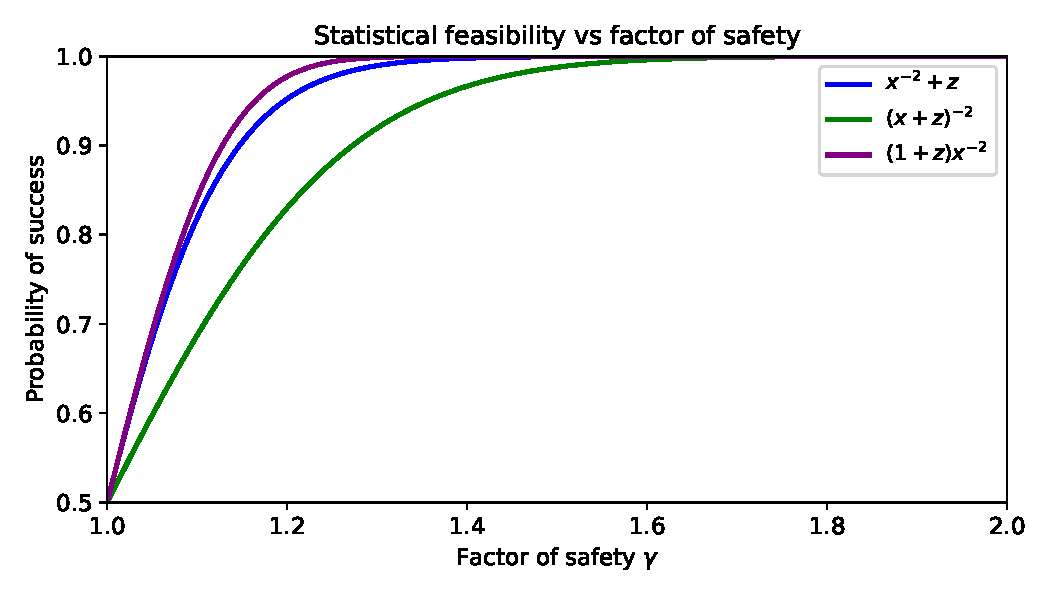
\includegraphics[width=0.60\textwidth]{stat_feasibility}\\
    {\small Probability of success vs factor of safety $\gamma$ for three uncertainty models}
  \end{center}
\end{frame}

\begin{frame}{The Six-Sigma Standard (Exercise 20.3)}
  \begin{columns}
    \column{0.50\textwidth}
      \begin{block}{Definition}
        \textbf{Six-sigma} requires that feasibility violations occur only when
        $|z| > 6\sigma$ (standard deviations):
        \[
          \Pr[g(\x,\z) \le 0] \ge 1 - \Pr[|z| > 6]
          \approx 1 - 1.973 \times 10^{-7}\%
        \]
      \end{block}
      \vspace{4pt}
      \textbf{Extremely stringent:} only $\approx 2\times10^{-9}$ of outcomes may violate.\\[4pt]
      \textbf{Six-sigma exercise:} Find $x^*$ such that $(x,z)$ feasible for all $|z| \le 6$:
      \[
        \text{minimize}\; x_1 \quad \text{s.t.}\; e^{x_1} \le x_2 + z \le 2e^{x_1}
      \]
      Solution: $x_1 = \ln 12 \approx 2.485$, $x_2 = 18$.
    \column{0.46\textwidth}
      \centering
      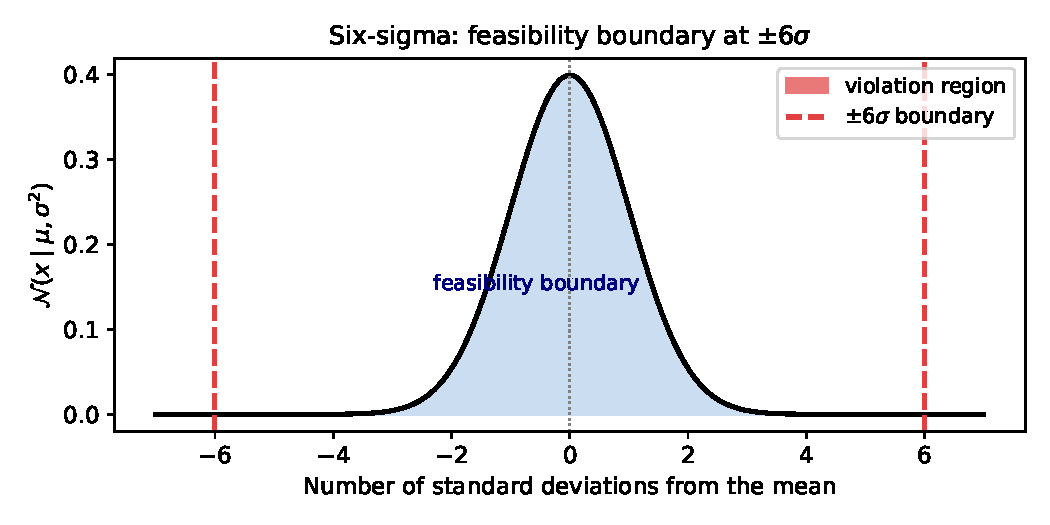
\includegraphics[width=\textwidth]{six_sigma}\\
      {\scriptsize Only tails beyond $6\sigma$ are infeasible (red)}
  \end{columns}
\end{frame}

\begin{frame}[fragile]{Python: Chance Constraints via Sample Average Approximation}
\begin{lstlisting}
import numpy as np
from scipy.optimize import minimize

np.random.seed(42)
N = 500  # number of scenarios

# Sample z ~ N(0, 0.01)  (sigma = 0.1)
z_samples = np.random.randn(N) * 0.1

def chance_constraint_violation(x, delta=0.05):
    """
    Returns fraction of scenarios that violate g(x,z) <= 1.
    Constraint: x^{-2} + z <= 1
    """
    g_vals = x**(-2) + z_samples
    violation_rate = np.mean(g_vals > 1.0)
    return violation_rate

# Minimize f(x) = x^2 subject to: Pr[x^{-2}+z <= 1] >= 0.95
# i.e., violation_rate <= 0.05
def objective(xvec):    return xvec[0]**2
def constraint(xvec):
    return 0.05 - chance_constraint_violation(xvec[0])

res = minimize(objective, [1.5],
               constraints=[{'type':'ineq','fun': constraint}],
               bounds=[(0.5, 5.0)], method='SLSQP')
print(f"Chance-constrained x* = {res.x[0]:.4f}")
print(f"Violation rate: {chance_constraint_violation(res.x[0]):.4f}")
\end{lstlisting}
\end{frame}

% ============================================================
\section{Summary \& Exercises}
% ============================================================

\begin{frame}[allowframebreaks]{Chapter 20 Summary}
  \begin{block}{Key Concepts}
    \begin{description}
      \item[Uncertain objective] $f(\x,\z)$ depends on uncontrollable $\z$
      \item[Set-based] $\z \in \Z$ — no distribution assumed
      \item[Probabilistic] $\z \sim P$ — distribution is modeled
    \end{description}
  \end{block}

  \textbf{Set-Based Methods:}
  \begin{itemize}
    \item \textbf{Minimax}: $\minimize_\x \max_{\z\in\Z} f(\x,\z)$\\
          Optimizes worst-case performance
    \item \textbf{Robust feasibility}: design feasible for \emph{all} $\z\in\Z$\\
          Robust set = intersection of feasible sets
    \item \textbf{Info-gap}: maximize robustness radius $\hat\eps(\x)$\\
          Requires a performance threshold $f_c$
  \end{itemize}

  \framebreak

  \textbf{Probabilistic Methods:}
  \begin{itemize}
    \item \textbf{Expected value}: $\minimize_\x \E_\z[f(\x,\z)]$\\
          Smooths landscape; shifts optima under input noise
    \item \textbf{Variance}: $\minimize_\x \Var_\z[f(\x,\z)]$\\
          Risk-neutral; combined with mean in practice
    \item \textbf{Mean-variance trade-off}: $\alpha\E[f] + (1-\alpha)\sqrt{\Var[f]}$\\
          Markowitz portfolio is the canonical example
    \item \textbf{VaR}: $\alpha$-quantile of objective\\
          Easy to understand; not coherent
    \item \textbf{CVaR}: expected value in worst $(1-\alpha)$ tail\\
          Coherent; tractable via Rockafellar-Uryasev formula
    \item \textbf{Chance constraints}: $\Pr[g(\x,\z)\le 0] \ge 1-\delta$\\
          Statistical feasibility; factor of safety approach
  \end{itemize}
\end{frame}

\begin{frame}[allowframebreaks]{Risk Measures Comparison}
  \begin{center}
  \begin{tabular}{lccc}
    \toprule
    \textbf{Method} & \textbf{Distribution?} & \textbf{Tail-sensitive?} & \textbf{Convex?}\\
    \midrule
    Minimax        & No  & Yes (worst-case) & If $f,\Z$ convex \\
    Info-gap       & No  & No (avg-case)    & Generally no \\
    Expected value & Yes & No               & If $f$ convex \\
    Variance       & Yes & Partially        & If $f$ convex \\
    VaR            & Yes & No (threshold)   & No \\
    CVaR           & Yes & Yes              & Yes \\
    Chance constr. & Yes & No (probability) & Special cases \\
    \bottomrule
  \end{tabular}
  \end{center}

  \framebreak

  \begin{block}{Choosing a Method}
    \begin{itemize}
      \item \textbf{Physical safety bound known} $\Rightarrow$ minimax or chance constraint
      \item \textbf{Distribution well-characterized} $\Rightarrow$ expected value or CVaR
      \item \textbf{Finance / risk management} $\Rightarrow$ CVaR (coherent, convex)
      \item \textbf{Engineering reliability} $\Rightarrow$ factor of safety or six-sigma
      \item \textbf{Trade-off desired} $\Rightarrow$ mean-variance (Markowitz)
    \end{itemize}
  \end{block}
\end{frame}

\begin{frame}{Exercises}
  \begin{block}{Exercise 20.1}
    Consider the objective shown below with three design points $a$, $b$, $c$.
    The objective is to minimize $\E_z[f(x+z)] - \sqrt{\Var_z[f(x+z)]}$.\\
    The optimal design is $x^* = a$ (minimizes both mean and std).
  \end{block}

  \begin{block}{Exercise 20.2: Factor of Safety — Beam Design}
    Minimize $f(x) = x^2$ (cross section area) subject to stress $g(x) \le \sigma_{\max} = 1$.\\
    Optimal: $x^* = \sqrt{\gamma}$. Three uncertainty models:
    \begin{enumerate}
      \item $g(x,z) = x^{-2} + z$ \quad (stress uncertainty)
      \item $g(x,z) = (x+z)^{-2}$ \quad (construction tolerance)
      \item $g(x,z) = (1+z)x^{-2}$ \quad (material property)
    \end{enumerate}
    \centering
    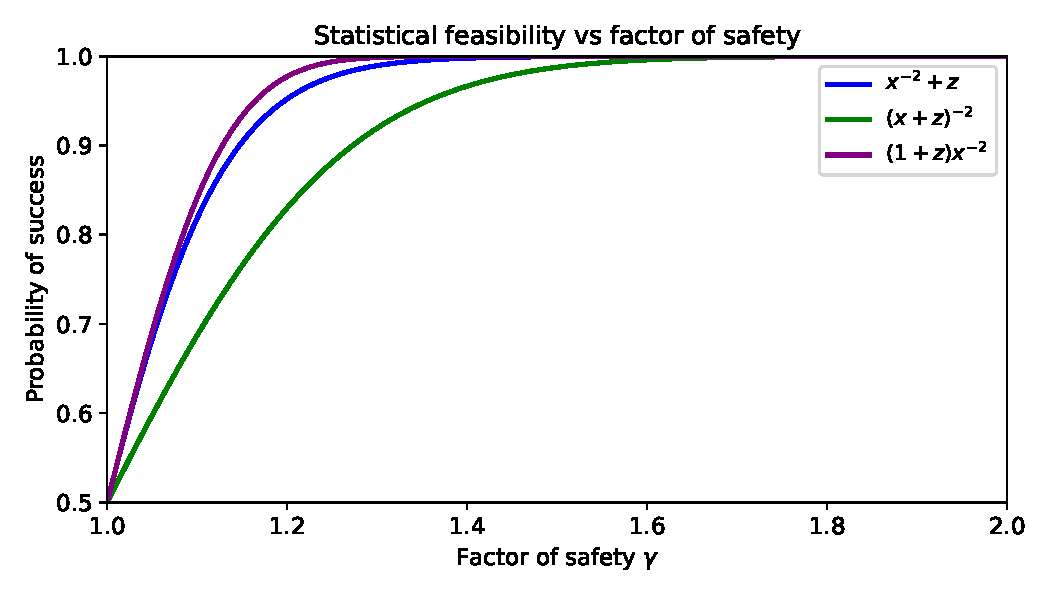
\includegraphics[width=0.50\textwidth]{stat_feasibility}
  \end{block}
\end{frame}

\begin{frame}{Exercise 20.3: Six-Sigma Feasibility}
  \begin{columns}
    \column{0.55\textwidth}
      \begin{block}{Problem}
        Minimize $x_1$ subject to:
        \[
          e^{x_1} \le x_2 + z \le 2e^{x_1}, \quad z \sim \Norm(0,1)
        \]
        Find $x^*$ such that $(x,z)$ is feasible for all $|z| \le 6$.
      \end{block}
      \textbf{Solution:}\\
      $x_2$ must satisfy $x_2 - z \ge e^{x_1}$ and $x_2 + z \le 2e^{x_1}$ for all $|z|\le 6$.\\[4pt]
      \textbf{Robust choice:} $x_2 = 1.5 e^{x_1}$ (center of $[e^{x_1}, 2e^{x_1}]$).\\[4pt]
      Width of feasible window: $e^{x_1}$; must accommodate $12\sigma$:
      \[
        e^{x_1} \ge 12 \;\Rightarrow\; x_1 = \ln 12 \approx 2.485
      \]
      \[
        x_2 = 1.5 e^{x_1} = 18
      \]
    \column{0.42\textwidth}
      \centering
      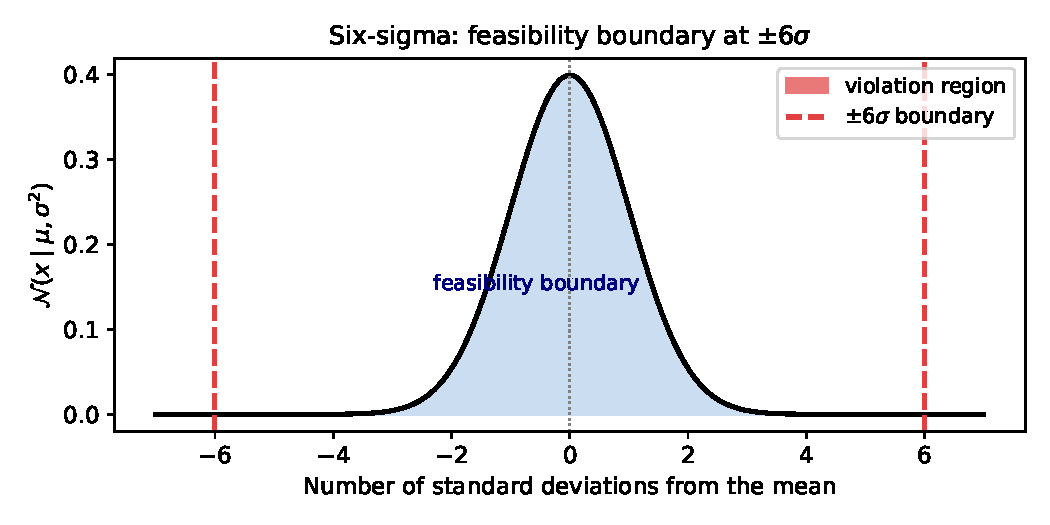
\includegraphics[width=\textwidth]{six_sigma}
  \end{columns}
\end{frame}

\begin{frame}{Conclusions}
  \begin{columns}
    \column{0.58\textwidth}
      \begin{block}{Key Takeaways}
        \begin{itemize}
          \item Uncertainty is \emph{inherent} in real-world optimization
          \item \textbf{Set-based} methods (minimax, info-gap) require no
                probability model — robust but often conservative
          \item \textbf{Probabilistic} methods use distributional information —
                more efficient when distribution is known
          \item \textbf{CVaR} is preferred over VaR: coherent, convex, tractable
          \item \textbf{Chance constraints} directly specify reliability requirements
          \item Methods can be combined (e.g., CVaR with chance constraints)
          \item Monte Carlo sampling enables optimization for any distribution
        \end{itemize}
      \end{block}
    \column{0.38\textwidth}
      \centering
      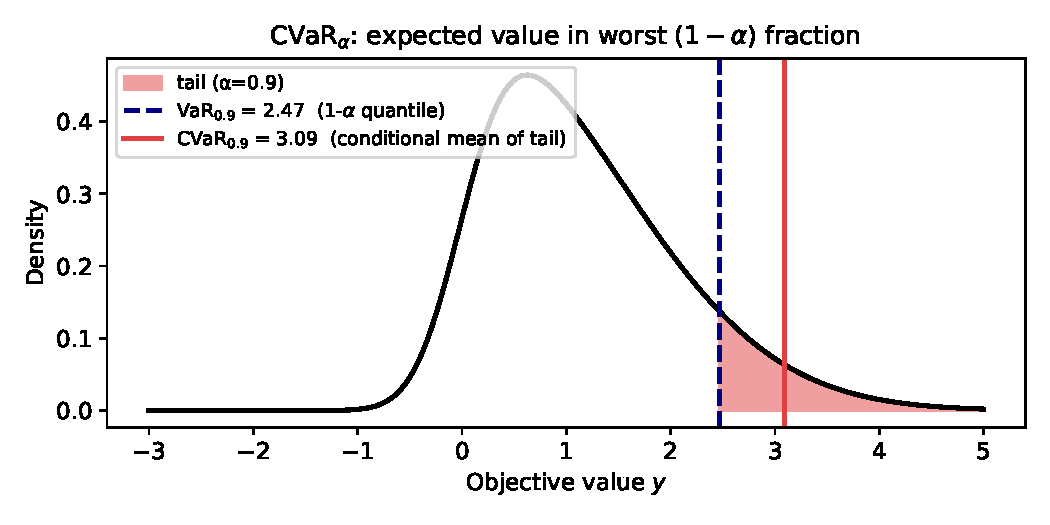
\includegraphics[width=\textwidth]{cvar_quantile}\\[4pt]
      {\small CVaR captures what VaR misses:\\severity of extreme outcomes.}
  \end{columns}
  \vspace{10pt}
  \centering
  {\Large\textbf{End of Chapter 20}}
\end{frame}

% ============================================================
\end{document}
